%%%%%%%%%%%%%%%%%%%%%%%%%%%%%%%%%%%%%%%%%%%%%%%%%%%%%%%%%%%
% EPFL report package, main thesis file
% Goal: provide formatting for theses and project reports
% Author: Mathias Payer <mathias.payer@epfl.ch>
%%%%%%%%%%%%%%%%%%%%%%%%%%%%%%%%%%%%%%%%%%%%%%%%%%%%%%%%%%%
\documentclass[a4paper,11pt,oneside]{report}
% Options: MScThesis, BScThesis, MScProject, BScProject
\usepackage[MScProject,lablogo]{EPFLreport}
\usepackage{xspace}
\usepackage[footnotes,hybrid]{markdown}
\usepackage{multirow}

\title{Design, implementation and evaluation of a fork accountability\\solution in the Tendermint consensus protocol}
\author{Andrea Piccione}
\supervisor{Dr. Dragos-Adrian Seredinschi}
\adviser{Prof. Rachid Guerraoui}
%\coadviser{Second Adviser}
\expert{Jovan Komatovic}

\begin{document}
\maketitle

\begin{abstract}

In this report we discuss the fork accountability problem, which concerns the detection of nodes responsible for a fork in a distributed network of machines running BFT consensus when the system is compromised. We analyze and study such a challenge in the context of the Tendermint protocol, whose consensus algorithm does not currently have any mechanism to make all replicas accountable for their actions in the case of a fork when more than one-third of machines in the system are faulty.

We are going to focus on describing the design of a fork accountability solution for Tendermint consensus algorithm, that was conceived by researchers from the École Polytechnique Fédérale de Lausanne and Informal Systems. This solution can guarantee the detection of faulty processes responsible for a fork in a completely asynchronous system. The core contribution of this work consists in validating this proposal with a proof-of-concept implementation where the algorithm was developed and tested along with several features. Finally, some benchmarks and experiments have been carried out in order to give the idea of the computational complexity of the solution from a performance point of view.

\end{abstract}

\maketoc

%%%%%%%%%%%%%%%%%%%%%%
\chapter{Introduction}
%%%%%%%%%%%%%%%%%%%%%%

Tendermint is a partially synchronous protocol which provides a simple and efficient algorithm to solve the problem of Byzantine fault-tolerant (BFT) consensus in a distributed network of processes. As every other BFT consensus protocol, the Tendermint algorithm relies on the assumption that byzantine processes are limited to a certain threshold: this assumption allows correct processes to have enough voting power to approve new blocks and guarantees the correctness and validity of the blockchain throughout the entire execution of the protocol. 

When this assumption cannot be ensured, malicious processes can cause the failure of the algorithm and create deviations from the main chain (better known as forks). In such cases, a failover solution should provide some reliable guarantees that, under certain constraints, allow the consensus algorithm to recover from the fault, detect the faulty processes responsible for a fork and eventually restore the conditions for the safe execution of the consensus algorithm.        

We define this problem as fork accountability and we present and analyze the conditions, the challenges and the consequences given by this inconsistency in Tendermint. In order to properly introduce the reader to the topic, an overview of the Tendermint protocol is presented before diving into the fork accountability problem (Chapter 2). 

This work proposes a fork accountability algorithm that solves such a problem without making any assumption on the communication model: we are going to describe its design and details by analyzing the possible attack scenarios and the variety of challenges faced and the trade-offs made during the study of such a solution by the researchers from the École Polytechnique Fédérale de Lausanne and Informal Systems (Chapter 3). 

In order to get a more practical idea of the potential of the designed solution, this project aimed at implementing the accountability algorithm in a simplified environment that gives the possibility to run experiments and test the application with different configuration and settings (Chapter 4). 

Thanks to the flexibility and modularity of the developed project, it has also been possible to evaluate the accountability algorithm in terms of computational resources and get a better idea of its performance (Chapter 5). 

We conclude this report with some interesting aspects and topics related to the fork accountability problem which could be further studied and analyzed in future work (Chapter 6). 

The main contribution of this thesis is a working implementation of a fork accountability solution validated from a theoretical and practical point of view. The implementation also offers promising results in tests along with good performance overall and can potentially offer a solid and well-founded contribution to the development of a fork accountability algorithm in the production Tendermint code.

%%%%%%%%%%%%%%%%%%%%
\chapter{Tendermint protocol overview and the fork accountability problem}
%%%%%%%%%%%%%%%%%%%%

\begin{markdown}

We are going to present a short and simple overview of the Tendermint protocol and the main aspects that are required to understand the fork accountability problem.
This is not an exhaustive and formal discussion about the Tendermint consensus protocol. We invite the reader to read the Tendermint documentation~\cite{tendermint-doc} and the official paper~\cite{buchman2018latest}.

## Tendermint consensus algorithm

[Tendermint](https://tendermint.com) is a partially synchronous Byzantine fault-tolerant (BFT)~\cite{wiki:bft} consensus protocol. The protocol requires a fixed set of *n* processes that attempt to come to a consensus on one value or, more precisely, on a block (a block is a list of transactions) using gossip-based communication. 

Tendermint is notable for its simplicity and performance and is currently one of the most mature and widely used implementations of BFT consensus.

### Properties 

The Tendermint consensus algorithm guarantees the following properties~\cite{buchman2018latest}, with respect to a consensus instance:

- **Agreement**: no two correct processes decide on different values

- **Validity**: a value decided is a valid value, with respect to the specifications of message validity

- **Termination**: all correct processes eventually decide

- **Integrity**: no correct process decides more than once in a single height 

In order to ensure all these properties, the Tendermint consensus algorithm assumes a correct majority of processes such that less than one-third of processes are faulty (*f*):
 
    n > 3f
 
When a process *p* is faulty, *p* can behave in an arbitrary way and we have no assumptions or guarantees regarding its actions.
 
In order to simplify the whole discussion, we assume the following from now on:
 
    n = 3f + 1

### Overview

As we can see in Figure 2.1, the consensus algorithm proceeds in rounds: in each round there is a validator (i.e., a process participating in the consensus) that proposes a value (proposer) and all the validators then vote during the round on whether to accept the proposed value or move on to the next round.

We can summarize the execution in a round in **two voting steps**: PREVOTE and PRECOMMIT steps. A vote can be for a particular value or for *nil* (null value). During a round, processes can exchange different types of messages, each one with a specific purpose:
 
- **PROPOSAL message**: sent by the proposer of the round to propose a value in a new round

- **PREVOTE message**: sent by validators to vote for a value during the first voting step

- **PRECOMMIT message**: sent by validators to vote for a value during the second voting step

A correct process decides on a value *v* in a round *r* upon receiving a proposal and quorum of at least *2f + 1* PRECOMMIT messages for *v* in a round *r*. 
A correct process sends a PRECOMMIT message for a value *v* in a round *r* upon receiving a proposal and a quorum of at least *2f + 1* PREVOTE messages for *v* in a round *r*~\cite{buchman2018latest}.

Validators wait some time before sending a PREVOTE for *nil* if they do not receive a valid proposal after a certain time (*proposalTimeout*) and they send a PRECOMMIT message for *nil* if they do not receive at least *2f + 1* matching PREVOTE messages for a value after a certain time (*prevoteTimeout*).
If processes do not receive at least *2f + 1* matching PRECOMMIT messages for a value after a certain time (*precommitTimeout*), they move to the next round~\cite{tendermint-overview}.

After a decision has been made, processes continue to agree on other values on another consensus instance (*height*) and they repeat the process described above in order to agree on different blocks.

\end{markdown}

\begin{figure}[h]
\centering
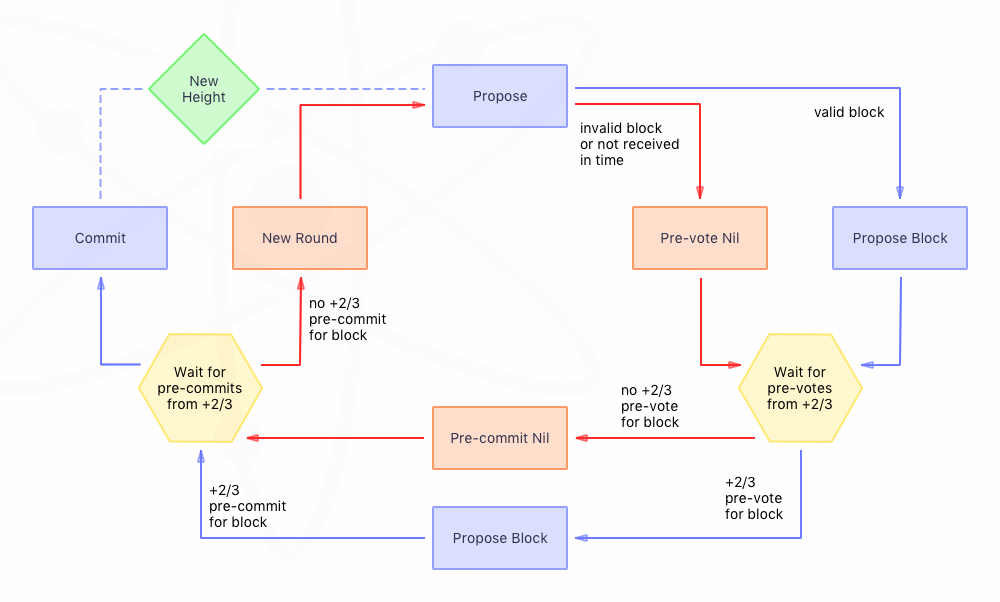
\includegraphics[scale=0.45]{tendermint_schema.png} 
\caption{Overview of the Tendermint consensus algorithm~\cite{tendermint-schema}.}
\label{fig:subim1}
\end{figure}

\begin{markdown}

### Rules

In order to ensure that processes will eventually come to a decision, there are some constraints that are applied. These rules aim at preventing any malicious attempt to cause more than one block to be committed at a given height. 

When a validator *p* sends a PRECOMMIT for a value *v* at round *r*, we say the *p* is *locked* on *v*. Validators can propose and send PREVOTE messages for a value they have locked and they can only change the locked value if they receive a more recent proposal with a quorum of PREVOTE messages. 

These conditions ensure both the safety and liveness properties of the consensus algorithm since a validator cannot send a PRECOMMIT message without a valid justification.

## Agreement property

We present the agreement property of the Tendermint protocol because it is important to properly frame the fork accountability problem. In this section, we also give a simple proof of the agreement property and show that it is not possible to violate the agreement property in Tendermint if there are at most *f* faulty processes.

### Idea behind the proof

As said before, we assume for simplicity that *n = 3f + 1*.
The key idea behind the proof of the agreement property is that any two sets of *2f + 1* processes have at least one correct process in common~\cite{buchman2018latest}.

Since there are two sets of *2f + 1* processes, their sum can be written as:
 
    2(2f + 1) = 4f + 2 = 3f + 1 + f + 1 = n + f + 1
     
That means that the intersection of these two sets contains at least *f + 1* processes or, in other words, at least one correct process.  

Given this result, we can easily prove the impossibility of having two sets of *2f + 1* PREVOTE or PRECOMMIT messages in the same round *r* for different values. If we assume the opposite by contradiction, then it would be possible to have at least *f + 1* processes that sent both the messages, which would mean *f + 1* processes are faulty. But at most *f* processes can be faulty in Tendermint, so the contradiction.

Moreover, at most one value can be locked in a round and, if a correct process decided value *v* in round *r*, *v* will be locked for all the next rounds after *r* on that height. This ensures that it is not possible to have another quorum for committing another value different than *v*.

### Proof

In order to formalize the above idea, we present a simple formal proof of the property.

Assume that a correct process *p* decides value *v* in round *r* and height is *h*. We want to prove that any other correct process *p'* in some round *r' >= r* of height *h* decides *v'* such that *v'* = *v*.

We have two cases:

- if *r' = r*: 

    *p'* has decided value *v'* in round *r*, therefore it has received at least *2f + 1* PRECOMMIT messages for value *v'* in round *r*. 
    Similarly, *p* has decided value *v* in the same round *r*, therefore it has received at least *2f + 1* PRECOMMIT messages for value *v* in round *r*. 
    As it has been shown previously, any two sets of *2f + 1* messages intersect in at least one correct process. Since a correct process only sends a single PRECOMMIT message, it must be that *v = v'*.  

- if *r' > r*:
        
    *p* has decided value *v* in the same round *r*, therefore it has received at least *2f + 1* PRECOMMIT messages for value *v* in round *r*.
    Since the number of faulty processes is at most *f*, at least *f + 1* correct processes have locked value *v* by round *r* and, by algorithm locking rules, they will send PREVOTE messages only for value *v* or *nil* in subsequent rounds of height h.
    
    In a similar way, *p'* has decided value *v'* in round *r' > r*, so it has received at least *2f + 1* PRECOMMIT messages for value *v'* in round *r' > r*. 
    Since the number of faulty processes is at most *f*, at least *f + 1* correct processes have locked value *v'* by round *r' > r* and these processes must have received at least 2f + 1 PREVOTE messages for value v' by round r'.
    
    From the fact that the intersection of *2f + 1* processes has at least one correct process, at least one correct process that locked value *v* in round *r* also sent a PREVOTE message for value *v'* in a later round *r' > r*. 
    Since this is impossible, it can only be that *v = v'*.

Since these are the only two possible cases, the above reasoning proves that the agreement property is satisfied.

### Guarantees 

As said before, the Tendermint consensus protocol is a simple and efficient algorithm that guarantees the four properties mentioned above. These properties are valid as long as faulty processes are at most one-third of the total number of validators in the system.

However, when this assumption is broken, processes can decide on different values in the same consensus instance and the blockchain can potentially diverge into two potential decision paths, making the entire protocol break.

Although it is not possible to ensure all the four properties in this scenario, it is necessary to have additional "safety" guarantees that allow the system to self-recover from the possible fault. The problem of fork accountability deals with this situation and will be addressed in the next section.

## Fork accountability

The agreement property of the Tendermint consensus algorithm can be violated if there are more than *f* faulty processes in the system, as previously discussed. When this situation occurs, more than one block can be decided in a single height and the protocol rules are violated. Since it is not possible to prevent this situation when the limit on the number of faulty processes in the system is exceeded, we aim at identifying faulty processes and banning them from the set of validators in order to re-establish a normal situation. We present such a problem, known as fork accountability, in more detail in this section.  

### Definition

A **fork** is a split in the blockchain network or, in other words, a divergence into different block paths~\cite{wiki:fork}. 
A fork happens when two correct validators decide on different blocks in the same height~\cite{fork-accountability-overview} (i.e., there are two commits for different blocks in the same consensus instance). 

In the context of the Tendermint protocol, a fork happens in height *h* when a quorum of messages (at least *2f + 1* PRECOMMIT messages) are sent for different values: more formally, there are two sets of at least *2f + 1* PRECOMMIT messages, A and B, such that A's messages are PRECOMMIT votes for value *v* and B's messages are PRECOMMIT votes for value *v' $\neq$ v* in height *h*.

The Tendermint consensus algorithm guarantees that a fork (i.e., a violation of the agreement property) cannot happen when the number of faulty processes is less than one third.
We want to address and analyze the problem of defining a Tendermint consensus algorithm that provides the same four properties (validity, agreement, termination, integrity) when the number of faulty processes is less than one third and guarantees, in addition, an efficient detection of faulty processes responsible for a fork when there are more than one-third of faulty validators.

In particular, we assume there are more than one third of faulty validators such that the following holds:

    f < num. faulty processes <= 2f

In the Tendermint protocol, all processes should be accountable for their actions and faulty validators should be identified and punished according to the protocol specifications, for example by removing them from the validators set.
We aim to give incentives to validators to behave correctly according to the protocol specifications and detect faulty validators, without mistakenly detecting correct validators. 
 
### Attack scenarios
 
In the previous section, we mentioned that a process can make the consensus fail with a fork. There are, indeed, multiple reasons that can generate a fork in the blockchain, all coming from processes that deviate from the protocol specification in various ways.

We can summarize some of the most important misbehaviors~\cite{fork-accountability-overview} that can possibly cause a fork in a consensus instance according to the Tendermint consensus algorithm rules: 

- a process sends multiple proposals in a round *r* for different values 

- a process sends a PREVOTE/PRECOMMIT message for an invalid value *v* in a round *r*

- a process sends multiple PREVOTE/PRECOMMIT messages in a round *r* for different values (**equivocation**)

- a process sends a PREVOTE/PRECOMMIT message for a value *v* despite having a lock on a different value *v'* (**amnesia**)

- a process sends a PRECOMMIT for a value *v* without having received at least two thirds PREVOTE messages for *v* 

\end{markdown}

\begin{figure}[h]
\centering
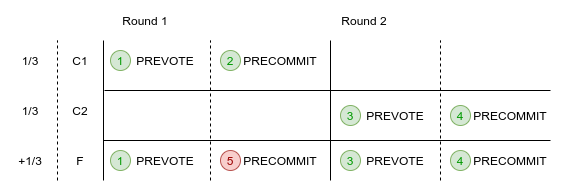
\includegraphics[scale=0.8]{fork_scenario.png} 
\caption{Schema of an amnesia attack~\cite{amnesia-attack}.}
\label{fig:subim1}
\end{figure}

\begin{markdown}

Figure 2.2 shows an example of a possible scenario where an amnesia attack~\cite{amnesia-attack} can occur.
C1 and C2 are two blocks of correct validators, F is a set of at least *f + 1* faulty processes.

In the first round, C1 and F send PREVOTE messages for value *v* and C1 only send PRECOMMIT for *v*. 
In the second round, C2 and F send PREVOTE messages for value *v'* (*v $\neq$ v'*) 
and both blocks send also PRECOMMIT messages for value *v'* (so, *v'* is committed).
Then, faulty processes decide to go back and send PRECOMMIT messages for *v* in the first round despite the fact they should be locked on *v'* and this clearly creates a fork in the main chain.

\end{markdown}

%%%%%%%%%%%%%%%%
\chapter{Design of a fork accountability algorithm}
%%%%%%%%%%%%%%%%

\begin{markdown}

The goal is to develop an accountability algorithm that analyzes the messages received by validators during an execution of a consensus instance and, therefore, is able to determine which processes respected the protocol and which ones did not and caused a fork. 
In order to convince all processes of the faultiness of a validator, we also want to show the proof of the misbehavior of malicious processes with respect to the Tendermint consensus protocol.

In other words, we want to design an accountable Tendermint algorithm. An accountable algorithm is one that:

- solves the consensus problem if the number of Byzantine processes is at most f

- if disagreement happens, then every correct process outputs a list of at least f + 1 faulty processes.

We assume that messages exchanged in the consensus algorithm are signed and it is not possible to forge messages (i.e., some process *p* cannot state that it has received a message from process *p'* if p' did not send that message or *p* did not receive it).

## Requirements

### Interface

The algorithm exposes the following interface (in the event of a fork):

- **detect(P)**: process P is faulty according to the accountability algorithm

Hence, all the processes that are detected are faulty. Some faulty processes could still be undetected because they were not responsible for a fork, even though they were faulty[^2].

### Properties

The algorithm guarantees the following properties:

- **accuracy**: if the accountability algorithm detects a process *p*, then process *p* is faulty

- **f+1-completeness**: the accountability algorithm eventually detects at least *f + 1* different processes

## Monitor

We want all correct processes to run the accountability algorithm and produce the same output (i.e, the faulty processes to ban from the validator set). We can abstract this concept and, instead of referring to every single correct process, we refer to a single entity that all validators know. We introduce a trusted third-party verification entity, called **monitor**, which is responsible to run the accountability algorithm~\cite{fork-accountability-specs}. In practice, everything the monitor does is carried out by every single correct process.

The monitor is responsible to coordinate and run the accountability algorithm as soon as a fork is detected. Since the input of the algorithm are the **message logs** of the validators (i.e., all the information related to the exchanged messages by processes in the consensus instance), the monitor will first request the message logs from each validator and then will run the accountability algorithm.

We assume that all validators keep track of all the messages they sent and received during an execution of the Tendermint consensus algorithm. 
The idea is that a correct process would be able to prove that it was not faulty by showing its activity (*message logs*) to the monitor.
The monitor should be able to detect all faulty processes that were responsible for generating a fork by analyzing the message logs from all the correct processes.

[^2]: In this case, the accountability algorithm can also detect other faulty behaviours that did not necessarily lead to a fork - this is a positive side effect.

## Fork scenarios

In order to better understand the problem, we analyze the scenarios when the fork can happen and how the monitor would be able to handle the situation when analyzing the log received from each validator~\cite{fork-scenarios}.

From now on, the expression "leading to a fork" will be used to generally define a set of misbehaviours that were responsible of a fork carried out by some malicious process. 
For example, saying "a process *p* leads to a fork" means that *p* caused a fork by having made one or more faulty behaviours in a specific consensus instance.

### Fork in a single round

A fork happens in a certain round *r* when two decisions are made in the same round *r* for different values.
In other words, this means that a correct process *p* had decided value *v* in round *r* and some other correct process *p'* (*p $\neq$ p'*) has decided value *v'* (*v $\neq$ v'*) in round *r*. 

Given the fact that all the messages that led to a fork have been exchanged in round *r*, at least *f + 1* processes must have sent a PREVOTE/PRECOMMIT message for both *v* and *v'*.
Since at least one correct process will receive the messages for both values, the monitor would be able to eventually identify the faulty processes that led to a fork.  

### Fork across different rounds

A fork happens in different rounds when two decisions for different values are made in different rounds. 
In other words, this means that a correct process *p* had decided value *v* in round *r* and some other correct process *p'* (*p $\neq$ p'*) has decided value *v'* (*v $\neq$ v'*) in round *r'* such that *r' > r*. 

Given this scenario, it can be noticed that at least *f + 1* processes have sent a PRECOMMIT message for value *v* in round *r* and also sent a PREVOTE message for value *v'* in round *r'* despite having locked value *v* when they sent a PRECOMMIT.

These processes are faulty unless they have a valid justification for sending the PREVOTE message for *v'* after being locked on *v* (i.e., other *2f + 1* PREVOTE messages for value *v'* in a round *r''* s.t. *r < r'' < r'*).
 
On the other hand, if they do have such a justification, it means that there are at least *f + 1* processes that sent a PRECOMMIT message for value *v* in round *r* and also sent a PREVOTE message for value *v'* in round *r''*, despite having locked value *v* when they sent the PRECOMMIT of round *r*.

It is clear that this scenario is similar to the one described at the beginning: the processes that sent a PREVOTE message for *v'* in *r''* are faulty unless they have a valid justification for sending the PREVOTE message for *v'* after being locked on *v*.

The monitor would be able to track down the origin of the misbehaviour by checking, recursively, that all the processes that sent a PREVOTE message for a value different from the one they were locked on have a valid justification.
Since messages cannot be generated out of anywhere, there must be an iteration of this recursive problem where the monitor would be able to find at least *f + 1* processes that sent a PREVOTE message without a valid justification and led to a fork.

In conclusion, only two possible options remain:

1. at least *f + 1* processes have sent both PREVOTE messages for value *v* and *v'* in the same round *r*

2. at least *f + 1* processes have sent a PRECOMMIT message for value *v* in round *r* and also sent a PREVOTE message for value *v'* in a round *r''* (such that *r < r'' <= r'*) without having delivered *2f +1* PREVOTE messages for value *v'* in a round *r'''* (where *r <= r''' < r''*)

## Challenges

### Handling invalid logs

Given the fact it deals with faulty processes, it is possible that the monitor received invalid message logs. An invalid message log is a message log which contains incomplete information regarding the actual messages sent and received by the owner of the log (this means some messages might have not been reported in the log).
Indeed, a faulty process is likely to alter and modify its message log in order to hide a possible misbehaviour. In that case, the monitor might not have enough information to detect all the faulty processes that led to a fork. 

Therefore, the following scenarios are possible~\cite{fork-accountability-specs}:
 
1. A process *p* denies having received a message *m* (*p*'s message log does not contain *m* as a message received)  

2. A process *p* denies having sent a message *m* (*p*'s message log does not contain *m* as a message sent) 

The first case can be safely ignored because it does not contribute to the generation of a fork.

The second point is instead more important in this discussion because a process can deny having sent a message *m* in order to hide its misbehavior. 
However, if *m* led to a fork, at least one process *p'* (*p $\neq$ p'*) received *m*: the monitor can add this missing message in *p*'s message log without needing to take any further action and simply correct the invalid message log received. 

From now on, the expression "inferring a message log" will be used to define the action carried out by the monitor to correct an invalid message log with the missing messages taken from other message logs received by *p*.

To summarize, the monitor can infer the valid message logs for each process after receiving the message logs from all the correct processes, which are guaranteed to arrive and to be correct.
Once all the message logs received are adjusted and corrected accordingly, the monitor can start analyzing each message log and determine whether the process owner of the message log is faulty or not.

### Communication model

The communication between the monitor and the validators for receiving message logs of the Tendermint consensus algorithm is a crucial aspect of the monitor execution.

The monitor needs to make sure it will receive the message logs from the correct processes and, depending on how the communication is modeled, some assumptions must be made in order to design a correct fork accountability algorithm.

#### Synchronous model

In the case of synchronous model, the monitor should wait a certain amount of time (*timeout*) to receive all the message logs before running the accountability algorithm.

After the *timeout*, if some process *p* did not send its message log, the monitor can only consider *p* faulty due to the nature of the communication, even though it does not have all the information to determine its misbehavior with certainty~\cite{fork-accountability-specs}. 
On the other hand, by not considering *p* faulty, the monitor might not be able to find at least *f + 1* faulty processes that led to a fork because the monitor could not have received enough message logs to determine the faultiness of at least *f + 1* validators after the *timeout* expiration.

#### Asynchronous model

The approach given above does not work in an asynchronous case, when there are no assumptions regarding the communication between the monitor and the validators. 

In fact, the monitor cannot expose some process *p* if it did not receive *p*'s message log: the monitor could mistakenly detect a correct process because it does not have enough information to determine if *p* had a valid reason to send a PREVOTE/PRECOMMIT message (in other words, accuracy property would be violated).
 
By receiving the message logs from other processes, the monitor can only determine if *p* equivocated. 
However, while analyzing the fork scenarios in the previous section, we have shown that faulty processes can lead to a fork by not equivocating. 

An asynchronous accountability algorithm can detect some process *p* only if *p* equivocated and, as a result, cannot detect a process *p* without having received the message log of *p*. Therefore, since a process can violate the agreement property by not equivocating, it is impossible the design of an asynchronous accountability algorithm in the current Tendermint consensus algorithm.  

In order to design a correct asynchronous accountability algorithm, it is necessary to slightly modify the Tendermint consensus algorithm so that the accuracy property of the accountability algorithm cannot be violated.

The critical case outlined above is when a process sends a PRECOMMIT message for a value *v* and then, in a later round, it sends a PREVOTE message for a different value than *v*. In this way, a faulty process can lead to a fork without making equivocation.

An asynchronous accountability algorithm would work correctly if processes can justify the sending of a PREVOTE message directly: a simple solution would be attaching the justifications to the PREVOTE message itself so that the accountability algorithm can directly check if the message has been correctly sent.
In this case, the monitor would be able to complete the accountability algorithm correctly (respecting both the completeness and accuracy properties) as soon as at least *f + 1* faulty processes will be detected and by relying on the fact that at least *f + 1* correct processes will send correct message logs.

## Algorithm design
 
Assuming the small modification in the Tendermint consensus algorithm described above, these are the high-level steps carried out by the monitor to run the asynchronous accountability algorithm:

1. upon a fork, the monitor requests message logs from all the validators

2. the monitor runs the accountability algorithm to detect faulty processes upon receiving at least *f + 1* message logs and at every new message log received when there are at least *f + 1* message logs 

3. while running the accountability algorithm, the monitor analyzes the received logs: for every message *m* that has been received by some other process but is not present in the sender's message log, the monitor attaches *m* to the message log of the sender of *m*

4. for each validator, the monitor scans the received message logs and the inferred message logs and determines for each process whether it is faulty or not by analyzing the history of sent messages and transitions

5. when the monitor detects at least *f + 1* faulty processes, the algorithm completes

Termination is guaranteed by the fact that correct processes will send their messages logs and their message logs will be correct (no sent message will be missing). 
If this condition does not hold, the algorithm would not be able to identify correctly all the faulty processes that led to a fork. 

Few final notes regarding the design of this algorithm:

- the monitor needs to analyze the message logs from the round of the first decision to the round of the second decision. However, validators will send their entire message logs because they cannot know when a decision has been taken in the Tendermint consensus algorithm. 

- the accountability algorithm runs for a single instance of consensus (i.e., for a single height). However, it can be easily configured to support multiple heights by running the same single-height algorithm on different heights. 

\end{markdown}

%%%%%%%%%%%%%%%%%%%%%%%%
\chapter{Implementation of a fork accountability solution}
%%%%%%%%%%%%%%%%%%%%%%%%

\begin{markdown}

## Project overview

The project is available at the following Github repository: 

    https://github.com/mikanikos/Fork-Accountability. 

The repository provides a simple implementation of the Fork Accountability algorithm described in the previous chapter in the Go language but it also offers a modular set of packages and libraries that allow to run experiments and benchmark the algorithm implementation in a test environment with different fork scenarios~\cite{github-project}:

- a simple connection library to provide a high-level API for establishing connections and communicating among processes based on a client-server architecture; 

- an accountability algorithm implementation based on the theoretical specifications given by the research scientists of the DCL lab at [EPFL](https://www.epfl.ch/en/) and [Informal Systems](https://informal.systems/);  

- monitor implementation that represents the independent verification entity used to run the accountability algorithm;  

- validator implementation that represents the processes that participate in the Tendermint Consensus protocol; 

- sample test scripts to easily run experiments and benchmarks and test both the accountability algorithm and the interaction between monitor and validators.

### Architecture

The project is organized in several files and packages in order to guarantee modularity and extensibility and maintain at the same time a clear and simple structure.

The monitor (monitor package) is the entity responsible to run the accountability algorithm. It takes as input parameters:

- the path of a yaml configuration file which is necessary to initialize and configure the algorithm

- the (optional) path of a file that can be generated to provide detailed information about the whole execution and, especially, of the accountability algorithm

The monitor is responsible for opening connections with all the validators and initialize the request of the message logs (described below).

Validators (validator package) are simple processes that listen on a given port and each one has its own messages logs that are the result of the execution of the Tendermint consensus protocol. Message logs and listening port are initialized through a configuration file (different for every validator) along with a unique validator identifier.
Every message in the configuration file must be specified with all the corresponding information associated with it (type, round, height, senderID, possible justifications).

The monitor will use the connection library to request message logs from all the addresses (i.e., validator processes) given in the config file. It will wait for responses from each validator and, as soon as a packet arrives, it will store and send it to the main thread. The main thread will run the fork accountability algorithm if enough messages have been received until that time.
The monitor will repeat the request after a timeout expires and if the message received is not valid. If the validator closes a connection or crashes, the monitor will stop waiting for packets from it and will notify the main thread about the failure in the reception.

The validator, after receiving a valid request packet, will respond back if it will have the message logs requested. Otherwise, it will just ignore the request and will not answer the monitor. Optionally, it's possible to configure a response to immediately inform the monitor about the missing log in order to save resources.

The main accountability algorithm is implemented in the accountability package and is deeply described in the documentation files of the docs folder. Please refer to for a theoretical background or for implementation-specific details.

The connection library implemented in this project wraps the well-known [net library](https://golang.org/pkg/net/) and provides some abstractions to establish a TCP connection, send and receive TCP packets, serialize and de-serialize messages and listen to a specific port.
This library is used by the monitor and the validator to exchange packets for both the request and the sending of the message logs.

### Structure

Overall, this is the current structure of the project:
    
- .github: contains Github Actions continuous integration config files

- accountability: contains the main accountability algorithm

- cmd: contains the binaries for the monitor and the validator. Inside each binary folder, there's a folder with sample config files. 

- common: contains abstractions used throughout the project to better handle the input of the algorithm;

- connection: contains the connection library used by monitor and validators to communicate.

- docs: contains markdown files documenting the project and the accountability algorithm from a slightly more theoretical perspective; 

- scripts: folder used to group scripts for running experiments and benchmarks in different scenarios;

- benchmarks: folder used to save the output of benchmarks experiments;

- report: folder that contains the latex files of this report;

- utils: utilities used for parsing configuration files and for testing the several functionalities of the modules implemented;

Every package that contains go files also has corresponding tests in `*_test.go` files. The README.md file contains detailed instructions to set-up the environment and run both experiments and tests.

The repository provides also Docker images packages available at the Github Package Registry, which allow using the monitor and the validator in a pre-configured environment. 

\end{markdown}

\begin{markdown}

## Monitor algorithm

In order to simplify the later discussion, we introduce some abstractions that help to better identify and classify the message logs received and handled by the monitor.

### Main abstractions

Each **Message** contains the following information:

- **Type** of the message, *type*

- **Unique identifier** of the sender of the message, *id*

- **Round** of the message, *r*

- **Value** of the message, *v*

A **Vote Set** is the set of all Messages that a process sent and received in a specific round *r*.

A **Height Vote Set** is the set of all Vote Set in a specific height *h* or the set of all Messages that a process sent and received in a specific height *h*.

Tendermint messages have several other important fields that are used by the consensus protocol for other purposes. However, we limit the scope of our discussion to this information only since they are essential for running the designed accountability algorithm.       

### Algorithm steps
 
These are the detailed steps of the execution of the monitor to run the asynchronous accountability algorithm: 
 
1. upon a fork, the monitor sends a request for validators' height vote sets (following a specific communication protocol) for a given height. The monitor starts waiting for incoming message logs.

2. the validators receive the request from the trusted monitor and they send whatever they have to the monitor immediately. 

3. the monitor runs the accountability algorithm upon receiving a new message log but only when **the total number of different height vote sets received is at least *f + 1***. 
If the threshold is met, the monitor runs the accountability algorithm. Otherwise, the monitor keeps waiting for other packets from the processes that did not reply yet. 
      
4. the accountability algorithm runs in two consecutive phases.

    1. **Pre-processing phase**: given the received message logs so far, the monitor "infers" the missing sent messages and attaches them to the original sender's height vote set.

    2. **Fault-detection phase**: the monitor scans the height vote set from the first round to the last round and checks that the rules of the Tendermint consensus algorithm are violated. If a process violates any of the Tendermint consensus algorithm rules, it is detected as faulty. 

    The output of the accountability algorithm is the list of processes that have been detected as faulty and the proof of their misbehaviour.
  
5. if the monitor detected **at least *f + 1* faulty processes** during the last execution of the accountability algorithm, the monitor completes. Otherwise, it keeps waiting for more height vote sets.

## Accountability algorithm

### Pre-processing phase
During this phase, the monitor analyzes all the height vote sets received. 
For each height vote set, the monitor scans all the received vote sets. 
For every message *m* in the received vote set, the monitor checks if the message is present in the set of messages sent by the sender of *m*. If it is not present, the monitor adds it to the sender's vote set.   

### Fault-detection phase
During this phase, the monitor analyzes each height vote set after the pre-processing phase and determines whether the process is faulty or not.
For every height vote set received, the monitor goes through all the sent messages in each round r from the first round to the last round. The monitor checks for the following faulty behaviours:

- the process equivocated in round r (sent more than one PREVOTE or PRECOMMIT message)

- the process sent a PRECOMMIT message but did not receive *2f + 1* valid PREVOTE messages to justify the sending of the PRECOMMIT message

- the process sent a PREVOTE message and did not have *2f + 1* valid PREVOTE messages as justification inside the PREVOTE

If one or more of these faulty behaviours is found in any of the rounds analyzed, the process is detected as faulty.

Please note that height vote sets that have not been received (therefore, they have been inferred during the pre-processing phase) will be checked for equivocation only.

## Pseudo-code implementation

We now present a simple pseudo-code version of the algorithm in order to make readers better understand some implementation details.
The following algorithm is only a high-level overview of the main steps of the accountability solution implemented, we invite the reader to check out the code for further details.  

### Monitor algorithm

The monitor has the following interface:

- **runMonitor(V, h, firstRound, lastRound)**: run the accountability algorithm on the set of validators V for height *h* from *firstRound* to *lastRound*, return the list of faulty processes in height *h*

In order to simplify the understanding of the algorithm, the algorithm uses the following high-level methods to model the communication between the monitor and validators:

- **sendRequest(v, h)**: send a request for the height vote set of height h to validator v 

- **deliverHVS()**: deliver the next incoming height vote set sent by some validator, return the next height vote set received

We present here below a simplified pseudo-code of the actual  implementation:

    // Monitor algorithm
    runMonitor(V, h, firstRound, lastRound):
        
        // compute max number of faulty processes
        // with respect to the number of validators  
        f = (V.length - 1) / 3
        
        // send request to validators
        for v in V:
            sendRequest(v, h)
        
        // store delivered height vote sets
        hvsDelivered = []
        
        // wait to deliver f+1 different height vote sets
        do:
            hvs = deliverHVS()
            hvsDelivered = hvsDelivered + hvs
        while (hvsDelivered.length < f+1)
        
        // run accountability algorithm
        faultyProcesses = runAccountability(hvsDelivered, firstRound, lastRound)
        
        // repeat until we find at least f+1 faultyProcesses
        while (faultyProcesses.length < f+1):
        
            // wait to deliver more HVS
            hvs = deliverHVS()
            hvsDelivered = hvsDelivered + hvs
        
            // run accountability algorithm 
            faultyProcesses = runAccountability(hvsDelivered, firstRound, lastRound)    
           
            
        // return the final output of the algorithm that satisfied exit condition
        return faultyProcesses

### Accountability algorithm

The following is the accountability algorithm used by the monitor to detect faulty processes based on the information given.

The accountability algorithm has the following interface:

- **runAccountability(hvsDelivered, firstRound, lastRound)**: run accountability algorithm on the height vote sets list *hvsDelivered* from *firstRound* to *lastRound*, return the list of faulty processes detected based on the parameters

The algorithm uses the following high-level methods for simplifying the presentation:

- **getHVSFromSender(hvsDelivered, id)**: get the height vote set corresponding to the sender *id* given, return *nil* otherwise 

- **newHvs(id)**: create a new height vote set given an *id*, return the newly-created inferred height vote set

- **getVoteSetFromRound(hvs, r)**: get the vote set from the given height vote set *hvs* of round *r*, return the vote set relative to the height vote set *hvs* given

We present here below a simplified pseudo-code of the actual  implementation:
    
    // Accountability algorithm
    runAccountability(hvsDelivered, firstRound, lastRound):
    
        // Pre-processing phase
                
        // go through all the height vote sets received
        for each hvs in hvsDelivered:
            // go through all the messages received
            for each m in hvs.received:
                // get height vote set of the sender of the message m
                hvsSender = getHVSFromSender(hvsDelivered, m.sender)
                
                // if not present in the height vote sets received, create it 
                if hvsSender == nil:
                    hvsSender = newHvs(m.sender)
                    // add inferred flag for later processing
                    hvsSender.inferred = true
                    hvsDelivered = hvsDelivered + hvsSender 
                
                // if m is not present in the hvs of the sender, add it
                if m is not in hvsSender:
                    hvsSender = hvsSender + m
                    
        // Fault-detection phase
        
        // set of faulty processes detected, duplicates are discarded
        faultyProcesses = []
        
        // go through all the height vote sets received
        for each hvs in hvsDelivered:
            // from the first to the last round    
            for each round r from firstRound to lastRound: 
                // get vote set from round
                vs = getVoteSetFromRound(hvs, r)
                
                // check for equivocation
                if vs.sent contains more than one PREVOTE or PRECOMMIT in round r:
                    faultyProcesses = faultyProcesses + hvs.sender                
                
                // if the hvs was not inferred, check for correctness of the execution
                // in round r according to tendermint consenus algorithm rules  
                if !hvs.inferred:
                    
                    // check if process sent a PRECOMMIT or a PREVOTE without proper
                    // justiifcation (PREVOTE messages must contain valid justifications) 
                    if vs.sent contains a PRECOMMIT/PREVOTE without a valid justification:
                        faultyProcesses = faultyProcesses + hvs.sender
                        
                        
        return faultyProcesses
        
                
## Implementation-specific details

- The communication between the monitor and the validators is over TCP and is structured as a normal client-server interaction.  

- The monitor checks the received responses for validity and does not accept a height vote set if this is not valid and will keep waiting for a valid response from validators. 
The monitor also keeps track of the received responses: if a validator sent a valid height vote set, the monitor will stop waiting for a response and closes the connection.
If some implementation failure is detected by the monitor (network failure, validator crashes before sending height vote set, etc.) the monitor will know that it will not receive a response from the failed validator. 
Therefore, the monitor will stop the execution if a response is not expected from any other process. 

- For the safety of the execution, the monitor has a timeout that aims at preventing a "wait-forever" state in case of some problems (network issue, invalid height vote set, error in config files, etc.). The timeout is not necessary from a theoretical point of view since the assumptions made guarantee that the accountability algorithm will eventually complete.

\end{markdown}


%%%%%%%%%%%%%%%%%%%%
\chapter{Evaluation and benchmarks}
%%%%%%%%%%%%%%%%%%%%

\begin{markdown}

The environment where the experiments have been carried out is a cloud virtual machine instance on [Google Cloud](https://cloud.google.com/), located in the zone us-central1-a. 
The machine type is a [n1-standard-16](https://cloud.google.com/compute/docs/machine-types#n1_standard_machine_types) (16 vCPUs, 60 GB memory), running the latest Ubuntu 20.04 LTS. The main hardware specifications and details are reported in Table.

The reported benchmarks consist of several executions of the monitor algorithm, both asynchronous and synchronous version, in different fork scenarios and interacting with different configurations of validators.
The fork scenarios are always due to validators sending a PRECOMMIT message without enough PREVOTE messages and have been automatically generated with a script that allows creating valid configuration files for both the monitor and the validators with user-defined parameters.

The parameters chosen for the benchmarks are the number of validators and the number of rounds between the first and the second decision in the fork. 
The Table summarizes the configurations used for the experiments.

The metrics used to evaluate the performance are the following:

- the execution time of the last (and successful) iteration of the accountability algorithm only

- the total elapsed time between the start and the end of the entire command used to execute the monitor algorithm (it includes the whole accountability algorithm plus connection and packet exchange with validators)

- the CPU utilization percentage of the command used to execute the monitor algorithm

- the maximum resident set size (RSS) allocated for the process running the command used to execute the monitor algorithm~\cite{wiki:rss}

The last three metrics have been computed using the [time command](https://en.wikipedia.org/wiki/Time_(Unix)) in its [extended version](https://man7.org/linux/man-pages/man1/time.1.html).

The benchmark experiments have been repeated three times with very similar results, therefore the obtained data can be considered moderately valid and reliable.

\end{markdown}


\begin{markdown}

## Total execution time

As we can see, the amount of time taken to run the entire monitor algorithm is relatively small in almost all cases. 
As expected, a higher number of both validators and rounds increases the time to complete the algorithm: there are not only more iterations (i.e., more messages) to execute in the accountability algorithm but there is also the overhead due to the communication between monitor and validators.

Even though validators have been set up to send back their message logs as soon as they receive the request, the communication protocol (which includes the connection establishment with each validator, the time to send/receive a packet to/from another process, etc.) has an impact on the data analyzed. 
This is also the reason why we notice that the number of validators has a greater impact on the time while the number of rounds minimally affects the results, especially for lower values.

We can notice that the synchronous version has slightly better performance overall than the asynchronous one: this is likely the result of the several executions of the accountability algorithm that must be run every time a new message log from a validator is delivered and there are at least *f + 1* message logs, as long as at least *f + 1* faulty processes are found. 
On the other hand, the synchronous version runs once when the timer expires or when all the expected message logs are received.   

\end{markdown}

\begin{table}[]
\centering
\begin{tabular}{l|c|c|c|c|c|c|}
\cline{2-7}
                  &  & \multicolumn{5}{c|}{Num. rounds} \\ \cline{2-7} 
\multirow{7}{*}{} & Num. validators & 1   & 10   & 100  & 500  & 1000  \\ \cline{2-7} 
                  & 4               & < 0.01 & < 0.01  & < 0.01 & < 0.01 &  0.01       \\ \cline{2-7} 
                  & 10              & < 0.01   & < 0.01   & < 0.01  & 0.01  &  0.01     \\ \cline{2-7} 
                  & 50              & 0.02    & 0.03     & 0.07      &  0.06    & 0.13      \\ \cline{2-7} 
                  & 100             & 0.12    & 0.29     & 0.18     & 0.19     &   0.56    \\ \cline{2-7} 
                  & 250             & 0.40    &  1.67    & 1.25     & 3.53      & 2.71      \\ \cline{2-7} 
                  & 500             &  1.43   &  39.36    & 12.74     &  32.46    &  17.31     \\ \cline{2-7} 
\end{tabular}
\caption{Total elapsed time (in seconds) between the start and the end of the monitor algorithm Unix process in asynchronous mode}
\end{table}


\begin{table}[]
\centering
\begin{tabular}{l|c|c|c|c|c|c|}
\cline{2-7}
                  &   & \multicolumn{5}{c|}{Num. rounds} \\ \cline{2-7} 
\multirow{7}{*}{} & Num. validators & 1   & 10   & 100  & 500  & 1000  \\ \cline{2-7} 
                  & 4               & < 0.01  & < 0.01  & < 0.01 &  < 0.01 & 0.01      \\ \cline{2-7} 
                  & 10              & < 0.01    & < 0.01     &   < 0.01   & 0.01  & 0.02      \\ \cline{2-7} 
                  & 50              & 0.03    &  0.02    & 0.03     &  0.06    &  0.08     \\ \cline{2-7} 
                  & 100             & 0.12  & 0.12    & 0.13  & 0.16     & 0.20      \\ \cline{2-7} 
                  & 250             &  0.63   & 0.62     &  0.69    &  0.68    &  1.02     \\ \cline{2-7} 
                  & 500             & 2.51    & 2.09     &  2.27    &  3.15    & 3.24      \\ \cline{2-7} 
\end{tabular}
\caption{Total elapsed time (in seconds) between the start and the end of the monitor algorithm Unix process in synchronous mode}
\end{table}


\begin{markdown}

## Execution time of the last iteration of the accountability algorithm

In order to better evaluate the accountability algorithm without the communication overhead, we measured the amount of time taken by the accountability algorithm during the last iteration (i.e., when the accountability algorithm completed successfully after receiving all the necessary message logs to detect the faulty processes).
Clearly, the accountability algorithm in the synchronous version always ran once, while we analyzed only the last execution of the accountability algorithm in the asynchronous version.

The outcome is similar to the one described in the previous section, where the higher number of validators and rounds makes the algorithm naturally a bit slower.
However, the number of validators has a more evident impact on the increase of the execution time, while the number of rounds continues to generally make a smaller difference unless the number is very high.

In this measurement the asynchronous case offers better results respect to the synchronous case because there are, in most cases, fewer message logs to analyze during the last execution.
in fact, the synchronous mode requires to run the algorithm when all messages logs have been delivered (or when the timeout has expired, but this case is not taken into consideration). 
On the other hand, the asynchronous version usually runs the last iteration of the accountability algorithm with a smaller number of message logs and, even though it carries out additional required computations (e.g. inferring the missing height vote sets, checking for justifications etc.) is a bit faster than the synchronous version, excluding the communication overhead.

\end{markdown}

\begin{table}[]
\centering
\begin{tabular}{l|c|c|c|c|c|c|}
\cline{2-7}
                  &  & \multicolumn{5}{c|}{Num. rounds} \\ \cline{2-7} 
\multirow{7}{*}{} & Num. validators & 1   & 10   & 100  & 500  & 1000  \\ \cline{2-7} 
                  & 4               & 126.877 & 127.291  & 181.153 & 146.343 & 296.025       \\ \cline{2-7} 
                  & 10              & 361.626   & 399.083   & 336.597  & 506.620  &  597.014     \\ \cline{2-7} 
                  & 50              & 4791.670    & 4033.630     & 5521.891      &  4800.140    & 8439.620      \\ \cline{2-7} 
                  & 100             & 24923.807    & 18204.071     & 17948.547     & 16754.867     &   23813.163    \\ \cline{2-7} 
                  & 250             & 136573.335    &  102765.305    & 101788.612     & 125541.701      & 116417.796      \\ \cline{2-7} 
                  & 500             &  521890.962   &  545614.360    & 448.957832     &  542385.895    &  454777.719     \\ \cline{2-7} 
\end{tabular}
\caption{Execution time (in microseconds) of the last iteration of the accountability algorithm in asynchronous mode}
\end{table}


\begin{table}[]
\centering
\begin{tabular}{l|c|c|c|c|c|c|}
\cline{2-7}
                  &   & \multicolumn{5}{c|}{Num. rounds} \\ \cline{2-7} 
\multirow{7}{*}{} & Num. validators & 1   & 10   & 100  & 500  & 1000  \\ \cline{2-7} 
                  & 4               & 115.766  & 160.097  & 135.614 &  382.94 & 435.577      \\ \cline{2-7} 
                  & 10              & 547.282    & 527.644     &   518.397   & 1119.330  & 1215.857      \\ \cline{2-7} 
                  & 50              & 1258.839    &  1000.103    & 10517.272     &  11943.328    &  16346.079     \\ \cline{2-7} 
                  & 100             & 51754.263  & 42.715984    & 42697.586  & 47.839259     & 55025.759      \\ \cline{2-7} 
                  & 250             &  325745.322   & 268818.704     &  267005.223    &  286744.539    &  311455.826     \\ \cline{2-7} 
                  & 500             & 1437563.693    & 1095183.626     &  1190059.827    &  1176744.325    & 1274205.946      \\ \cline{2-7} 
\end{tabular}
\caption{Execution time (in microseconds) of the last iteration of the accountability algorithm in synchronous mode}
\end{table}

\begin{markdown}

## CPU and memory utilization
Regarding the more technical metrics, the algorithm runs well without over-using too many computational resources.
CPU utilization has been measured by analyzing the percentage of CPU (respect to multiple cores) used by the monitor algorithm process.
Memory utilization has been measured by analyzing the amount of memory allocated to the monitor algorithm process.

Even under more "stressful" conditions, the algorithm does not require more than four cores and 500 megabytes to run.  
Apparently, the asynchronous mode requires slightly more cores but less memory to run. However, the results are machine-specific and they are not completely uniform across all the experiments carried out. 
Therefore, it is difficult to extract an exact trend for this data. However, we can say that for relatively high computations the algorithm works efficiently with a small amount of resources and is not expensive for limited machines.

\end{markdown}


\begin{table}[]
\centering
\begin{tabular}{l|c|c|c|c|c|c|}
\cline{2-7}
                  &   & \multicolumn{5}{c|}{Num. rounds} \\ \cline{2-7} 
\multirow{7}{*}{} & Num. validators & 1   & 10   & 100  & 500  & 1000  \\ \cline{2-7} 
                  & 4               & 133 & 175  & 200 & 137  & 166       \\ \cline{2-7} 
                  & 10              & 266   & 257   & 228  & 253  &  282     \\ \cline{2-7} 
                  & 50              & 384    & 312     & 258      &  426    & 327      \\ \cline{2-7} 
                  & 100             & 300    & 215     & 295     & 399     &   252    \\ \cline{2-7} 
                  & 250             & 500    &  242    & 273     & 202      & 255      \\ \cline{2-7} 
                  & 500             &  544   &  158    & 193     &  166    &  186     \\ \cline{2-7} 
\end{tabular}
\caption{CPU percentage utilization of the monitor algorithm Unix process in asynchronous mode}
\end{table}


\begin{table}[]
\centering
\begin{tabular}{l|c|c|c|c|c|c|}
\cline{2-7}
                  &  & \multicolumn{5}{c|}{Num. rounds} \\ \cline{2-7} 
\multirow{7}{*}{} & Num. validators & 1   & 10   & 100  & 500  & 1000  \\ \cline{2-7} 
                  & 4               & 150  & 175  & 160 & 171 & 123      \\ \cline{2-7} 
                  & 10              & 214    & 233     &  216   & 266  & 250      \\ \cline{2-7} 
                  & 50              & 321    & 375    & 359     &  421    &  540     \\ \cline{2-7} 
                  & 100             & 292  & 317    & 336  & 400     & 480      \\ \cline{2-7} 
                  & 250             &  358   & 407     &  316    &  434    &  334     \\ \cline{2-7} 
                  & 500             & 379    & 414     &  402    &  301    & 354      \\ \cline{2-7} 
\end{tabular}
\caption{CPU percentage utilization of the monitor algorithm Unix process in synchronous mode (a value greater than 100 means that more than one core has been utilized)}
\end{table}

\begin{table}[]
\centering
\begin{tabular}{l|c|c|c|c|c|c|}
\cline{2-7}
                  &  & \multicolumn{5}{c|}{Num. rounds} \\ \cline{2-7} 
\multirow{7}{*}{} & Num. validators & 1   & 10   & 100  & 500  & 1000  \\ \cline{2-7} 
                  & 4               & 5.884 & 5.904  & 6.132 & 6.384  & 7.552       \\ \cline{2-7} 
                  & 10              & 6.864   & 6.616   & 7.208  & 8.984  &  10.644     \\ \cline{2-7} 
                  & 50              & 12.772    & 14.452     & 17.060      &  20.120    & 26.448      \\ \cline{2-7} 
                  & 100             & 23.248    & 26.924     & 27.640     & 34.212     &   55.156    \\ \cline{2-7} 
                  & 250             & 70.768    &  90.164    & 92.548     & 115.196      & 152.024      \\ \cline{2-7} 
                  & 500             &  225.900   &  256.472    & 265.504     &  326.636    &  396.940     \\ \cline{2-7} 
\end{tabular}
\caption{Maximum RSS (in megabytes) of the monitor algorithm Unix process in asynchronous mode}
\end{table}


\begin{table}[]
\centering
\begin{tabular}{l|c|c|c|c|c|c|}
\cline{2-7}
                  &  & \multicolumn{5}{c|}{Num. rounds} \\ \cline{2-7} 
\multirow{7}{*}{} & Num. validators & 1   & 10   & 100  & 500  & 1000  \\ \cline{2-7} 
                  & 4               & 5.752  & 5.892  & 6.004 & 6.644 & 7.160      \\ \cline{2-7} 
                  & 10              & 6.628    & 6.552     &  6.828   & 9.516  & 10.780      \\ \cline{2-7} 
                  & 50              & 12.772    & 13.776    & 14.068     &  19.880    &  24.900     \\ \cline{2-7} 
                  & 100             & 21.520  & 23.356    & 24.616  & 33.904     & 43.852      \\ \cline{2-7} 
                  & 250             &  77.040   & 74.624     &  75.540    &  105.016    &  120.552     \\ \cline{2-7} 
                  & 500             & 243.324    & 248.952     &  248.584    &  287.856    & 365.908      \\ \cline{2-7} 
\end{tabular}
\caption{Maximum RSS (in megabytes) of the monitor algorithm Unix process in synchronous mode}
\end{table}


%%%%%%%%%%%%%%%%%%%%%%
\chapter{Related problems and future work}
%%%%%%%%%%%%%%%%%%%%%%

\begin{markdown}

Fork accountability is not the only problem that must be addressed when a fork occurs. Indeed, a reliable consensus algorithm should also provide guarantees on the detection and recovery from a fork, which are complementary problems to fork accountability. 

In this section, we analyze these two aspects and provide intuitive solutions to solve both problems in the Tendermint Consensus algorithm that could be further studied in future work. Moreover, we give some insights on possible improvements and developments of the fork accountability algorithm provided.

## Fork detection

A fork detection solution~\cite{failure-detection} aims at detecting a fork as soon as possible in a reliable and efficient way.

We define the following interface for a fork detection algorithm:

- **detect(h)**: a fork has occurred at height *h*

The fork detection algorithm guarantees the following properties:

- **accuracy**: if the accountability algorithm detects a fork at height *h*, then a fork occurred at height *h*

- **completeness**: if a fork occurred at height *h*, the algorithm eventually detects the fork

As already said regarding the fork accountability algorithm, we can assume that *n = 3f + 1* and that at most *2f* faulty processes are present in the system.

Since there are at most *2f* faulty processes in the system and the minimum quorum for a commit is *2f + 1*, when a fork occurs there is at least one correct process that took part in the quorum for the commit (i.e., at least one correct process must have sent a PRECOMMIT message for a value that was committed).

Instead of referring to every single correct process, we can keep referring to the monitor. A simple solution for the fork detection problem would be based on receiving notifications every time a commit is made in order to detect a possible fork.
Processes will notify the monitor every time a commit is made and will send the monitor the proof for the commit (i.e., at least 2f+1 valid PRECOMMIT messages). The monitor would be able to verify the validity of the commit and will detect a fork as soon as two valid commits will be received.

Once it has detected the fork, the monitor will start the fork accountability algorithm in order to detect the faulty processes, as described before.

Faulty processes are not able to make the algorithm fail because, as said before, at least one correct process will receive the commit and, consequently, will send it to the monitor. Even sending a fake commit to the monitor would not trick the monitor because it must contain at least 2f+1 valid PRECOMMIT messages that the monitor can verify.

A simple illustrative pseudo-code version of this idea is shown here below:


    // monitor initializes a map int -> bool that allows keeping track
    // whether a decision has already been made in a specific height
    init():
	    heightCommitMap = init(map: int -> bool s.t. returns false when no entry is present)

    // upon receiving at least 2f+1 precommit for height h from a process 
    deliverCommit(messageSet, height):
   
        // verify if the message sent is a valid commit
	    if verify(messageSet):
		    // check if this was the first decision for this height
		    if heightCommitMap[height]:
			    // fork has been detected
			    detect(height)
		    else:
			    heightCommitMap[height] = true

This is not meant to be a complete solution to the problem because it just provides a basic intuitive idea to handle the fork detection. It also lacks formal theoretical support which is required for the full refinement of the algorithm.
The validation and possible proof of concept of this algorithm is left to future work.

## Fork recovery

A fork recovery mechanism allows validators to agree on the state of the system after a fork occurred. 
This step should occur after validators have run the fork accountability algorithm and it includes the ban of faulty processes (detected by a fork accountability algorithm) from the validator set and the possible restart of the blockchain with the new validator set.

It is clear that the Tendermint consensus algorithm cannot proceed further without having enough correct validators, namely 4 validators, in order to make the algorithm work correctly. In fact, there is no quorum of at least *2f + 1* processes that allows satisfying the Tendermint consensus rules when there are only 4 validators in the system. 
Therefore, if the number of left processes after the banning phase is lower than 4, the consensus algorithm should block and should be able to restart only when another valid process will join the validator set based on the protocol rules.
Unless this case occurs, processes need to find a way to restart the system from a stable, common point such that invalid decisions and modifications due to the faulty configuration of the system are discarded.

The simplest idea to achieve this is giving validators the ability to save and restore the state of the system before a fork occurred.
In other words, processes should be able to save the current state of the blockchain and their internal state every time before starting a new consensus instance (new height). In this way, if a fork occurs at height h, processes would be able to restore their previous state before starting height *h* and re-execute the consensus instance of that height with the new correct validator set.

A simple illustrative pseudo-code version of this idea is shown here below:


    // each validator initializes a map int -> State, where State is a protocol-specific
    // type, that allows to keep track of the state before starting a new consensus instance
    init():
        validatorSet = getCurrentValidatorSet()
        heightStateMap = init(map: int -> State)

    // before starting a consensus instance, 
    // each validator saves the current system state and
    // start the new height as defined the Tendermint consensus algorithm
    startHeight(h):
        heightStateMap[h] = getCurrentSystemState()	

    // method executed after a validator received the fork accountability
    // output (faultyProcesses) about a fork on a certain height
    onForkAccountabilityCompletion(faultyProcesses, height):

        validatorSet = validatorSet - faultyProcesses

        if validatorSet >= MIN_CONSENSUS_PARTICIPANTS:
            restoreState(heightStatesMap[height])
            startHeight(height)
        else:
            throwError("The new set of validators doesn't have enough participants")
           
    // external methods and variables
    - getCurrentValidatorSet(): retrieves the current list of validators in the system
    
    - getCurrentSystemState(): retrieves the current state of the validator
    
    - restoreState(State): restore the validator state to the state given as parameter
    
    - MIN_CONSENSUS_PARTICIPANTS: defines the minimum number of validators
    allowed by the protocol
    

Although this solution could be considered valid at first, a future study should be dedicated to the complete validation and study of this algorithm.


## Fork accountability implementation improvements

As some readers might have noticed, the fork accountability problem can be easily solved by simply piggybacking justifications in every single message.
The reason why this solution has not being taken into consideration is its overhead: the amount of information to store and exchange among processes would be huge and this solution requires several changes to be applied directly to the Tendermint consensus algorithm. 

The proposed asynchronous accountability algorithm only requires including justifications in every PREVOTE message and fewer modifications of the Tendermint protocol than the above one.

However, this mechanism of including justifications can be implemented in different efficient ways: this project only offers a simple Proof of Concept of a possible high-level accountability solution.
For example, a possible efficient implementation can implement justifications in the form of signatures: processes can broadcast the justifications before sending a PREVOTE message and receive a signature from other processes as a result of the validation of the justifications sent. Future work on this project can focus on finding an efficient implementation of the monitor algorithm given in this work.  


## Fork tolerance
The fork accountability solution outlined in the previous sections relies on the monitor entity which is a centralized entity. It would be desirable executing the whole accountability algorithm among validators in order to eventually decide on which faulty processes must be banned from the validator set.

The problem is not trivial and it is not even certain that is solvable. 
Intuitively, processes need to run a distributed algorithm that allows reaching consensus on the faulty processes in the system.
However, the system itself is compromised because there are more than *f* faulty processes (i.e., there is not a quorum of correct processes that allows running the consensus correctly). The study and  design of a possible solution to such a problem could be further analyzed in future work.


\end{markdown}


%%%%%%%%%%%%%%%%%%%%
\chapter{Conclusion}
%%%%%%%%%%%%%%%%%%%%

In this work, we have tackled the fork accountability problem from different points of view in order to better show all the theoretical and practical implications this challenge offers. From a high-level perspective, we have concretely defined the problem, analyzed all the scenarios where the problem can occur and analyzed the main misbehaviors a process can do to create the conditions of a fork.

After tackling the problem, we described the design and the implementation of a fork accountability algorithm in Tendermint using the Go programming language. We showed how it is possible to implement an algorithm when the communication between the monitor and validators is completely asynchronous, made the different algorithmic parts more concrete and took steps into getting a sense of the validity and performance of this algorithm. We carefully studied and tested the proposed solution both from a correctness and a performance point of view, thanks to the numerous experiments and benchmarks that have been carried out, and proved that the algorithm is correct and efficient in terms of computational complexity. 

Although the proposed implementation is not a built-in and ready-to-use solution for Tendermint, it offers the high-level components and blocks that are fundamental for an integration of the fork accountability algorithm into production code. We also believe that this work can offer valid results for future work on a possible generalization of the fork accountability problem to different types of replicated services and an important starting point for developments of the related problems that have been outlined in Chapter 6.

\acknowledgments{I would like to thank Jovan Komatovic and Dragos-Adrian Seredinschi for providing all the theoretical background and advice during the development of the project (especially for sharing the design of the fork accountability algorithm they worked on), for all the comments and reviews of both code and documentation as well as the assistance given throughout the entire semester.}
\makeacks


\cleardoublepage
\phantomsection
\addcontentsline{toc}{chapter}{Bibliography}
\printbibliography

% Appendices are optional
% \appendix
% %%%%%%%%%%%%%%%%%%%%%%%%%%%%%%%%%%%%%%
% \chapter{How to make a transmogrifier}
% %%%%%%%%%%%%%%%%%%%%%%%%%%%%%%%%%%%%%%
%
% In case you ever need an (optional) appendix.
%
% You need the following items:
% \begin{itemize}
% \item A box
% \item Crayons
% \item A self-aware 5-year old
% \end{itemize}

\end{document}